\documentclass{article}
\usepackage[utf8]{inputenc}
\usepackage{fontawesome}
\usepackage{hyperref}
\usepackage{graphicx}
\usepackage{amsmath,amssymb}
\usepackage[left=2cm,right=2cm,bottom=2cm,top=2cm]{geometry}
\usepackage{float}


\title{Arquitectura de Computadoras Lab-2}
\author{anthony.aguilar }
\date{September 2020}

\begin{document}

\maketitle
\newpage
%\section*{Comentarios previos}
%\begin{itemize}
    \item Dentro de la carpeta de cada pregunta hay un makefile para compilar, ejecutar, mostrar las waves y limpiar los archivos generados al finalizar.
    \item Use github\faGithub \space porque trabaje este laboratorio en 2 computadoras y necesitaba una forma de compartir los archivos entre ambas. Y el repositorio es publico para que los links adjuntos funcionen.
\end{itemize}


\section*{Ejercicio 1}
\subsection*{Explicación}
Al analizar el comportamiento del Tlatch observamos que este invierte los valores de q y qn cuando t=1 y c=1.\\
En la implementación añadí un delay y un caso base para que no todos los valores de q y qn sean desconocidos al realizar a simulación. 

\subsection*{Tabla de verdad}
\begin{figure}[h]
    \centering
    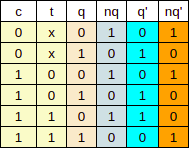
\includegraphics{fotos/TruthTable/arki-lab2-TT_tlatch.png}
\end{figure}

\subsection*{Mapa de Karnaugh}
\begin{figure}[h]
    \centering
    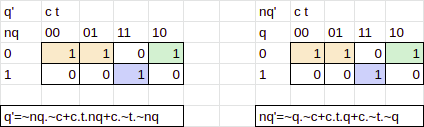
\includegraphics[scale=0.8]{fotos/kmaps/arki-lab2-kmap_tlatch.png}
\end{figure}
%\subsection*{Ecuaciones booleanas}

\newpage
\subsection*{Resultados}
\begin{figure}[htbp]
    \centering
    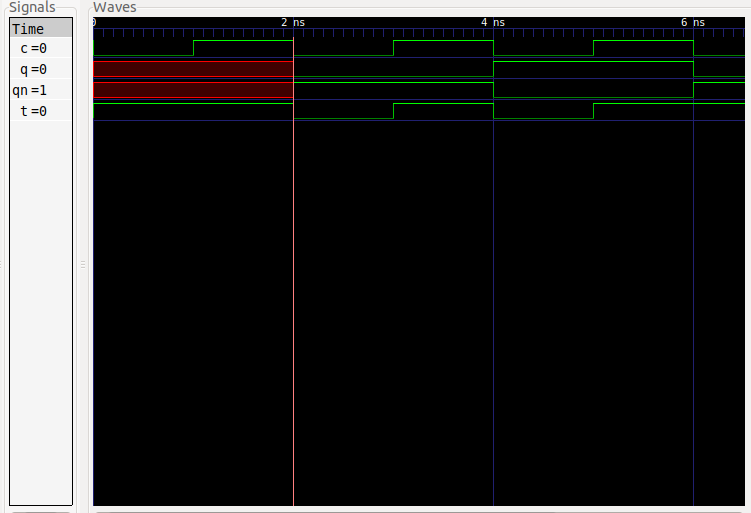
\includegraphics[scale=0.5]{fotos/resultados/arki-lab2-R_tlatch.png}
\end{figure}
\newpage

\section*{Ejercicio 2}
\subsection*{Explicación}
Al analizar el comportamiento del JKlatch observamos que este invierte los valores de q y nq cuando c=1, j=1 y k=1. Asigna los valores de j a q y de k a nq cuando j y k son diferentes ,y c=1. Y mantiene los valores previos de q y nq cuando j=0 y k=0 ,y c=1. Al igual que el T-latch en la implementacion le agregue un delay para evitar oscilaciones infinitas.

\subsection*{Tabla de verdad}
\begin{figure}[h]
    \centering
    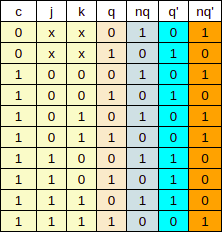
\includegraphics{fotos/TruthTable/arki-lab2-TT_jklatch.png}
\end{figure}
\subsection*{Mapa de Karnaugh}
\begin{figure}[h]
    \centering
    \includegraphics{fotos/kmaps/arki-lab2-kmap_jklatch.png}
\end{figure}
%\subsection*{Ecuaciones booleanas}

\newpage
\subsection*{Resultados}
\begin{figure}[h]
    \centering
    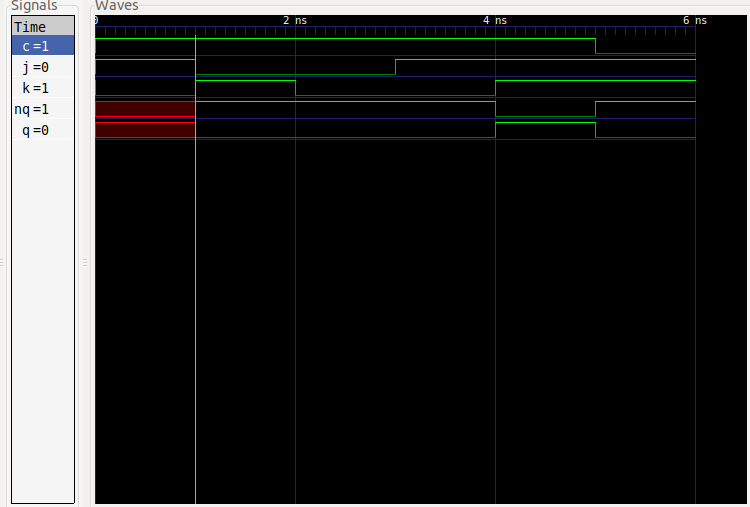
\includegraphics[scale=0.5]{fotos/resultados/arki-lab2-R_jklatch.png}
\end{figure}
\newpage

\section*{Ejercicio 3}
\subsection*{Explicación}
Un T-flip-flop hace lo mismo que un T-latch excepto que lo realiza en los posedge del clock.

\subsection*{Tabla de verdad}
\begin{figure}[h]
    \centering
    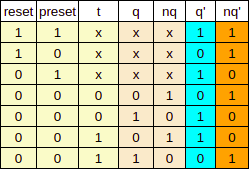
\includegraphics{fotos/TruthTable/arki-lab2-TT_tflipflop.png}
\end{figure}
%\subsection*{Mapa de Karnaugh}

%\subsection*{Ecuaciones booleanas}

%\subsection*{Resultados}
%\begin{figure}[h]
%    \centering
%    
%\end{figure}
\newpage

\section*{Ejercicio 4}
\subsection*{Explicación}
Un JK-flip-flop hace lo mismo que un JK-latch excepto que lo realiza en los posedge del clock.

\subsection*{Tabla de verdad}
\begin{figure}[h]
    \centering
    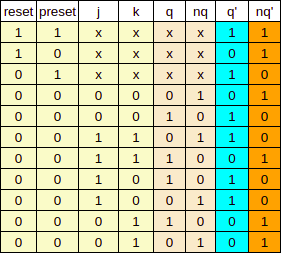
\includegraphics{fotos/TruthTable/arki-lab2-TT_jkflipflop.png}
\end{figure}
%\subsection*{Mapa de Karnaugh}
%\begin{figure}[h]
%    \centering

%\end{figure}

%\subsection*{Ecuaciones booleanas}


%\subsection*{Resultados}
%\begin{figure}[h]
%    \centering

%\end{figure}



\end{document}
